% Printed 468; principal PDF 475; Google PDF 479.
\par\clearpage
\noindent\makebox[0pt][l]{\fontsize{13}{16}\selectfont 468}\hfill{\small\textbf{CORRESPONDENCE.}}\hfill\null\par\medskip
\noindent would not occur until a few minutes later. If one then reads the scale and advances the alidade quickly, one can contrive to give the observer at the place towards which the light is thrown its full brilliance for more than 2 minutes. Clearly the effort is incomparably less if a third mirror is mounted directly on the large mirror, perpendicular to the plane of the sextant, at the inclination $a$. This turns the sextant into a complete sun mirror. It is markedly inferior only because the small telescope with only half the light does not reach very great distances and because the third mirror does not remain stationary when the sextant moves on its stand. I do, however, intend to have such a third mirror fitted to my sextant for return signals.

\par\noindent\hspace*{\parindent}The small trials made so far have gone as follows. \textls[120]{First}, merely on the observatory terrace, at a distance of 60 metres, the light was such that one could not look at it even for an instant without pain. \textls[120]{Second}, a little farther down, at a distance of 150 metres, looking at it for just a few seconds was painful to the eye. I made only these two trials myself, since I have as yet no one who could set up the instrument and I therefore had to do it myself. (It would be better to train someone else to do it were the stand not so imperfectly balanced that it must be handled with an extremely light touch if the trials are to succeed at all. Once there is a third mirror, this difficulty clearly disappears.) In the following trials, the observations were made in part by Professor \textsc{Ulrich}, who now holds an appointment here, and in part by Lieutenant \textsc{Hartmann}.

\par\noindent\hspace*{\parindent}In the \textls[120]{third} trial the distance was 300 metres. Professor \textsc{Ulrich} described the light as magnificent and as tiring to the eye when looked at steadily.

\par\noindent\hspace*{\parindent}The day before yesterday, \textls[120]{a fourth trial}, at a distance of 2000 metres. Professor \textsc{Ulrich} again called the light magnificent and compared it with 3 times the brilliance of Venus as it appears at night at its finest. His companion, he said, could hardly express his astonishment that such brilliance could be produced.

\par\noindent\hspace*{\parindent}Yesterday, \textls[120]{a fifth trial}, at the site of the future \textls[120]{south-}

% Printed 469; principal PDF 476; Google PDF 480.
\par\clearpage
\noindent\null\hfill{\small\textbf{HELIOTROPE.}}\hfill\makebox[0pt][r]{\fontsize{13}{16}\selectfont 469}\par\medskip
\noindent\textls[120]{ern} meridian mark, where I had to have a passage cut through a considerable stretch of woodland, at a distance of 11890 metres. Lieutenant \textsc{Hartmann} again calls the light \textls[120]{magnificent} and thinks that it probably equalled Venus in the evening twilight in intensity but was, as he put it, more \textls[120]{offensive} to the eye. It goes without saying that all these observations were made with the naked eye. A workman whom he had with him was so startled at the first flash that he cried fire. In the theodolite telescope the crosshair appeared completely severed at that sharp point of light.

\par\noindent\hspace*{\parindent}The mirror on my sextant measures exactly 2 Paris inches in width and $1\frac14$ inches in height. The mirror on the heliotrope made by \textsc{Rumpf} has nearly the same dimensions.

\par\noindent\hspace*{\parindent}I thought you might welcome news of these results. Until I have carried out further trials on a somewhat larger scale with the actual sun mirror, I would prefer that nothing of this get out.

\par\noindent\hspace*{\parindent}I now have every hope that this device will serve even at the greatest distances in my system of triangles. I believe that if the sun mirrors are built according to the second design indicated in my last letter, and the mirror is made sufficiently large, then the only limits henceforth on the lengths of the triangle sides will be those set by the spherical shape of the Earth.

\par\noindent\hspace*{\parindent}Perhaps these ideas can also find important applications in other respects, for example as signals for astronomical determinations of longitude, since this light can always be concealed and made to reappear in an instant. Perhaps they might even be used for other telegraphic signalling, at least when the sun shines somewhat steadily, if agreed meanings are assigned to precisely measured intervals between the light's appearances and disappearances.

\par\noindent\hspace*{\parindent}My Hohehagen signal was finished yesterday. I intend still this week (if \textsc{Rumpf} keeps his word) to complete both the difficult adjustment of the sun mirror and the measurement here of the angle Hohehagen-meridian mark, and then to set out for the Hohehagen.\enspace .\ .\ .\ .\ .\ .

% Printed 470; principal PDF 477; Google PDF 481.
\par\clearpage
\noindent\makebox[0pt][l]{\fontsize{13}{16}\selectfont 470}\hfill{\small\textbf{CORRESPONDENCE.}}\hfill\null\par\bigskip
\begin{center}{\large\textsc{Gauss} to \textsc{Schumacher}.\quad Göttingen, 11 July 1821.}\end{center}
\par\noindent\hspace*{\parindent}.\ .\ .\ .\ .\ .\enspace Perhaps a notice on my new instrument, which I would like to name the heliotrope, could serve as the opening contribution[\textsuperscript{*})]. I hope that this way of observing can become of the greatest importance to higher geodesy. At short distances (up to 2 miles), you could imagine no finer target than light reflected from a bright cloud. I hope reflected sunlight will provide the finest target at the very greatest distances.\enspace .\ .\ .\ .\ .\ .
\par\bigskip
\begin{center}{\large\textsc{Gauss} to \textsc{Schumacher}.\quad Göttingen, 8 November 1821.}\end{center}
\par\noindent\hspace*{\parindent}.\ .\ .\ .\ .\ .\enspace \textsc{Zach} has translated the article on the heliotrope in the Göttingischen gelehrten Anzeigen in his journal[\textsuperscript{**})]. There are several inaccuracies in the translation, however. One of the two new heliotropes is now finished. It gives a magnificent effect, but we have great difficulty getting good mirrors. Those we have had so far are extremely poor, which detracts little or nothing from the effect itself but makes adjustment very difficult. Yesterday I made a trial with moonlight. At a distance of about 250 metres, small though it was, it produced an exceedingly beautiful effect, a light like that of Venus (at night, when it is high) but many times more brilliant. I have developed telegraphing to a fair degree and can, if need be, give several thousand different signals.\enspace .\ .\ .\ .\ .\ .
\par\bigskip
\begin{center}{\large\textsc{Gauss} to \textsc{Schumacher}.\quad Steinkrug am Deister, 10 July 1822.}\end{center}
\par\noindent\hspace*{\parindent}.\ .\ .\ .\ .\ .\enspace This year I have 3 heliotropes proper and another heliotrope apparatus in operation. Two of the former are always working in the distance. It is a splendid thing (a luxury) to measure angles between two heliotrope lights on fine evenings, and the agreement of the results is then often quite admirable.\enspace .\ .\ .\ .\ .\ .
\par\medskip\noindent\rule{4cm}{.4pt}\par
\begingroup\footnotesize
\noindent\hspace*{\parindent}[\textsuperscript{*}) \textsc{Schumacher} had asked for a contribution to the Astronomischen Nachrichten.]\par
\noindent\hspace*{\parindent}[\textsuperscript{**}) Correspondance astronomique, géographique, etc. du Baron \textsc{de Zach}.\quad Vol. V.\quad 1821, pp. 374/382.]\par
\endgroup

% Printed 471; principal PDF 478; Google PDF 482.
\par\clearpage
\noindent\null\hfill{\small\textbf{HELIOTROPE.}}\hfill\makebox[0pt][r]{\fontsize{13}{16}\selectfont 471}\par\bigskip
\begin{center}{\large\textsc{Gauss} to \textsc{Schumacher}.\quad Göttingen, 15 January 1827.}\end{center}
\par\noindent\hspace*{\parindent}I return herewith the paper on the adjustment of heliotropes[\textsuperscript{*})]. Only as to the $3^{\mathrm{rd}}$ method for the $7^{\mathrm{th}}$ adjustment, if I remember rightly, did I actually have something different in mind from what is said here. I meant to set a sextant so that its mirrors are exactly parallel, with the index at the \textls[120]{true} zero point and, what really matters here, with the mirrors duly adjusted to be perpendicular to the plane of the sextant. One then holds the sextant so as to see directly the image of a bright, sharply defined object reflected in mirror component I (fixed stars of the first magnitude or a sufficiently distant heliotrope light would be better than the Sun), and to see the image from mirror component II by reflection in the two sextant mirrors, thus in effect after three reflections. Only one image should be seen. I admit, however, that I have never used this method myself. Its applicability also depends on the dimensions of the heliotrope and sextant. The distance between the centres of I and II must be somewhat smaller than the distance from the centre of the large sextant mirror to the axis of the telescope. So by all means leave it as it is
\begin{center}
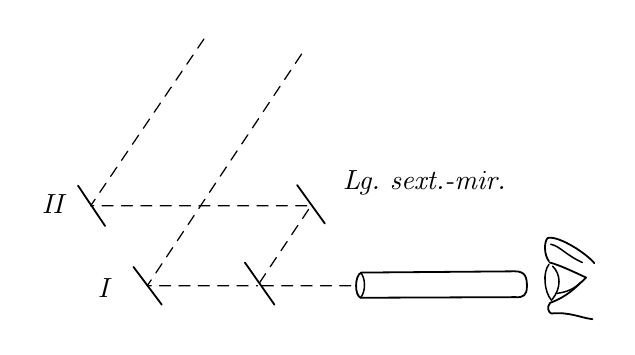
\begin{tikzpicture}[x=.008cm,y=-.008cm,line cap=round,line join=round]
\path[use as bounding box] (50,0) rectangle (970,475);
\draw[line width=.45pt,dash pattern=on 4pt off 3pt] (330,18)--(150,283)--(500,283)--(415,410)--(575,410);
\draw[line width=.45pt,dash pattern=on 4pt off 3pt] (485,42)--(240,410)--(415,410);
\draw[line width=.65pt] (130,251)--(173,315) (218,380)--(263,440) (478,250)--(522,311) (395,373)--(442,440);
\node[font=\itshape,anchor=east] at (122,280) {II};
\node[font=\itshape,anchor=east] at (194,414) {I};
\node[font=\itshape,anchor=west] at (535,247) {Lg.\ sext.-mir.};
\draw[line width=.65pt] (580,389)--(824,387)..controls (841,387) and (843,397)..(843,411)..controls (843,425) and (837,429)..(825,428)--(579,429)..controls (569,426) and (569,393)..(580,389);
\draw[line width=.55pt] (579,389)..controls (587,399) and (587,418)..(579,429);
\draw[line width=.65pt] (878,371)..controls (870,361) and (870,340)..(876,334)..controls (894,330) and (938,359)..(950,374);
\draw[line width=.55pt] (881,344)..controls (897,348) and (903,360)..(931,373);
\draw[line width=.65pt] (879,373)..controls (892,376) and (916,387)..(937,397)..controls (919,414) and (907,427)..(880,437)..controls (874,443) and (877,453)..(882,454)..controls (910,451) and (929,461)..(947,463);
\draw[line width=.55pt] (884,379)..controls (897,392) and (898,413)..(883,432);
\draw[line width=.55pt] (878,376)..controls (868,388) and (870,419)..(882,433);
\draw[line width=.55pt] (891,422)..controls (906,420) and (918,415)..(928,405);
\end{tikzpicture}
\end{center}
\noindent written, especially since each reader can easily supply the necessary precautions. For instance, it is best to set the mirror system so that the Sun is approximately in the plane to which the mirror axis is perpendicular. If some time elapses between the measurements on the two mirror components (more than a few seconds, which a skilful observer can probably avoid), one must allow for it.\enspace .\ .\ .\ .\ .\ .
\par\medskip\noindent\rule{4cm}{.4pt}\par
\begingroup\footnotesize\noindent\hspace*{\parindent}[\textsuperscript{*}) See the following paper.]\par\endgroup
\begin{center}\rule{3.5cm}{.4pt}\end{center}

% Printed 472; principal PDF 479; Google PDF 483.
\par\clearpage
\noindent\makebox[0pt][l]{\fontsize{13}{16}\selectfont 472}\hfill{\small\textbf{HELIOTROPE.}}\hfill\null\par
\vspace*{4.4cm}
\begin{center}
\begin{tabular}{c}\hline
\small\textbf{Astronomische Nachrichten, Vol. V, No. 116, February 1827, pp. 329--334.}\\\hline
\end{tabular}\par\bigskip
{\large The Adjustment of the Heliotrope.}
\end{center}
\par\noindent\hspace*{\parindent}The complete adjustment of the heliotrope requires eight operations in all.
\par\noindent\hangindent=1.8em\hangafter=1\hspace*{1em}1.\ 2.\quad The optical axis of the telescope is made parallel to its axis of rotation by means of the adjusting screws $E$ and $F$ (Fig. 1).
\par\noindent\hangindent=1.8em\hangafter=1\hspace*{1em}3.\quad The mirror axis $AB$ is set perpendicular to the axis of rotation of the telescope by means of the screws $CC$ (Fig. 1) on one arm of the fork that carries the mirror axis.
\par\noindent\hangindent=1.8em\hangafter=1\hspace*{1em}4.\ 5.\ 6.\quad The planes of the three mirrors (the smaller mirror and the two components of the larger one) are set parallel to the mirror axis by means of the screws $G$, $H$, $I$ (Fig. 2).
\par\noindent\hangindent=1.8em\hangafter=1\hspace*{1em}7.\quad Component II of the larger mirror is brought into a plane parallel to component I by means of the screw $K$ (Fig. 2).
\par\noindent\hangindent=1.8em\hangafter=1\hspace*{1em}8.\quad The small mirror must be set by means of the screw at its tail so that the plane of the mirror is perpendicular to the planes of both components of the large one.
\par\noindent\hspace*{\parindent}I pass over adjustments 1 and 2 as generally known.

\par\noindent\hspace*{\parindent}To carry out adjustment 3 entirely independently, I set the heliotrope on a firm pedestal, set the mirror axis $AB$ (Fig. 3) vertical with the stem $AD$ pointing down, and turn this stem until it is parallel to the axis of the telescope on the eyepiece side\textsuperscript{*}). All this by eye alone. From the stem $AD$ I suspend a not overly sensitive
\par\medskip\noindent\rule{4cm}{.4pt}\par
\begingroup\footnotesize\noindent\hspace*{\parindent}\textsuperscript{*}) This can also be done the other way around, mutatis mutandis.\par\endgroup

% Printed 473; principal PDF 480; Google PDF 484.
\par\clearpage
\noindent\null\hfill{\small\textbf{HELIOTROPE.}}\hfill\makebox[0pt][r]{\fontsize{13}{16}\selectfont 473}\par\medskip
\noindent spirit level, and bring the bubble \textls[120]{nearly} to centre by altering the length of the wires on which it hangs, then \textls[120]{exactly} to centre by means of the foot screws. I then turn the stem $180^\circ$ about the mirror axis, carefully lift out the telescope, and put it back in the opposite position (Fig. 4). The adjustment is unnecessary if the bubble again comes to centre. Otherwise half of the deflection is corrected at the foot screws and the other half at the screws $CC$ (Fig. 1). Returning to the previous position shows whether the division was made correctly. I pass over the precautions required in this procedure, since anyone will discover them without instruction and I subsequently used the procedure either not at all or only for the first rough adjustment\textsuperscript{*}).

\par\noindent\hspace*{\parindent}A procedure I have used for adjustments 4, 5, and 6 rests on the principle that a plane $ab$ (Fig. 5), by a half-turn about an axis $AB$ parallel to it, is brought from its initial position $ab$ into the parallel but opposite position $cd$. If the axis and the plane are not parallel, however, as in Fig. 6, the two positions $ab$ and $cd$ will not be parallel either. To test this on a mirror I set up two telescopes $M$, $N$ (Fig. 7) fitted with crosshairs, so that distinct objects $O$, $P$ appear on their optical axes and so that these axes nearly intersect, or lie nearly in one plane. Having removed the fork from the telescope and fixed it to a small box or board, I place the mirror to be tested on a table close to the intersection of the optical axes, so that the axis of rotation $AB$ lies approximately in their plane and bisects the angle between them. I then set the mirror $L$ perpendicular to that plane and, by small turns and gentle taps both on the mirror itself and on the box, make the image of $O$, reflected in the mirror, appear on the optical axis of $M$. I then turn the mirror $180^\circ$ about its axis and see whether in this position (Fig. 8) the image of $P$ appears on the optical axis of $N$. If this cannot be achieved by turning the mirror about the axis $AB$ alone, then one half must be corrected at the box and the
\par\medskip\noindent\rule{4cm}{.4pt}\par
\begingroup\footnotesize\noindent\hspace*{\parindent}\textsuperscript{*}) The applicability of this method moreover depends on one condition\rlap{\hspace{.05em}\raisebox{2ex}{.}}, that the cylindrical extensions by which the telescope rests in the bearings are of exactly the same thickness. Careful attention has been paid to this in the instruments made by Mr. \textsc{Rumpf}.\par\endgroup
\par\medskip\noindent\makebox[0pt][l]{\small IX.}\makebox[.86\linewidth][r]{60}\par

% Printed 474; principal PDF 481; Google PDF 485.
\par\clearpage
\noindent\makebox[0pt][l]{\fontsize{13}{16}\selectfont 474}\hfill{\small\textbf{HELIOTROPE.}}\hfill\null\par\medskip
\noindent other half by adjusting the position of the mirror relative to its axis. The objects $O$, $P$ need not be far away provided the mirror sits close to its axis. I placed them at a distance of about 70--80 feet.

\par\noindent\hspace*{\parindent}Several means are available for making adjustment 7. The simplest, which also provides sufficient accuracy, is to look at a straight line approximately parallel to the mirror axis in the two halves of the large mirror. It must appear as a straight line there, which the naked eye can judge with great accuracy.\ \raisebox{.55ex}{.}\ I used the facade of the observatory for this. --- A second method is to observe a fine object (a heliotrope light) with a telescope with a large objective (a comet seeker) in both mirrors at once, and adjust component II until only one image is seen. Clearly this also gives adjustment 6 if 5 has already been made. --- A third method is to take the altitudes of the Sun with a sextant using the two components of the large mirror as artificial horizons. The altitudes must be equal once the adjustment is made. --- A fourth method will present itself directly.

\par\noindent\hspace*{\parindent}For making the $8^{\mathrm{th}}$ adjustment, I have found the following procedure best. I set up the heliotrope and an auxiliary telescope with crosshairs so that the optical axis of the latter is parallel to that of the heliotrope telescope, in the same vertical plane and higher by about half the distance between the centres of the two components of the large mirror (Fig. 9). I do this by pointing the heliotrope at a clearly visible distant object, taking out the telescope, and putting it back in the reverse position once the auxiliary telescope at the specified height has been pointed at the same object. The mirror axis is then set vertical, with component I uppermost. By turning the mirror system, and the telescope as well if necessary, I make an object appear by reflection in the small mirror on the optical axis of the heliotrope telescope. If the same object appears by reflection in component I of the large mirror on the optical axis of the auxiliary telescope, the plane of the small mirror makes a right angle with that of component I. Otherwise the tail screw is used to make the necessary

% Printed 475; principal PDF 482; Google PDF 486.
\par\clearpage
\noindent\null\hfill{\small\textbf{HELIOTROPE.}}\hfill\makebox[0pt][r]{\fontsize{13}{16}\selectfont 475}\par\medskip
\noindent correction. Adjustment 7 can then also be tested in the same way by turning the heliotrope telescope $180^\circ$ about its axis so that component II comes uppermost. Objects on the other side must clearly be chosen for this.

\par\noindent\hspace*{\parindent}The methods described so far are all independent of one another, with the sole restriction that 7 must be carried out after 6 because touching the screw $I$ would affect adjustment 7. For adjustment 3, however, if 4 has already been made, or for both at once, I have used a procedure based on the principle that a surface turned about an axis perpendicular to it always remains in the same plane. Hence, if the small mirror is set perpendicular to the axis of the heliotrope telescope (which can be done in either of two ways, by turning the reflecting surface \textls[120]{toward} or \textls[120]{away from} the telescope), the image of any object must remain stationary in this mirror while the telescope is turned about its axis. I therefore set the small mirror perpendicular to the axis of the telescope, initially by eye, with the reflecting surface facing away from the objective (Fig. 10). I make the setting more exact by first judging with the naked eye whether the image of an object to one side stays motionless as the telescope is turned about its axis. I then set up an auxiliary telescope with crosshairs, with the mirror axis vertical, so that the image of some object to one side, reflected in the small mirror, appears on the optical axis of the auxiliary telescope, and so that this axis is directed nearly at the centre of the small mirror. I now give the heliotrope telescope a half-turn about its axis and see whether the reflected image has remained on the optical axis of the auxiliary telescope. If it has not, half the deviation to the left or right is corrected by turning the mirror system, and half the deviation upward or downward at the screws $CC$ (Fig. 1). The auxiliary telescope\textsuperscript{*}) is pointed again so that the reflected image appears exactly on the optical axis. A further half-turn of the heliotrope telescope about its axis will then show whether the division was made correctly. The plane of the small mirror $ab$ (Fig. 11) is thus now exactly perpendicular to the axis of the telescope,
\par\medskip\noindent\rule{4cm}{.4pt}\par
\begingroup\footnotesize\noindent\hspace*{\parindent}\textsuperscript{*}) Or the heliotrope, though this cannot be done conveniently without assistants.\par\endgroup
\par\medskip\noindent\makebox[.86\linewidth][r]{60\textsuperscript{*}}\par

% Printed 476; principal PDF 483; Google PDF 487.
\par\clearpage
\noindent\makebox[0pt][l]{\fontsize{13}{16}\selectfont 476}\hfill{\small\textbf{HELIOTROPE.}}\hfill\null\par\medskip
\noindent so that if adjustment 4 has already been made, 3 is also exact. If, however, the plane of the small mirror is not parallel to the axis $AB$ (Fig. 11), it cannot be brought into an opposite position perpendicular to the axis of the telescope by turning the mirror system. At the greatest deviation it will differ from that position by twice its inclination to the mirror axis (Fig. 12). Repeat the previous experiment in this position, taking an object in a direction that makes an obtuse angle with the axis of the telescope (Fig. 13). If the mirror is now set so that the reflected image, which initially appeared on the optical axis with the mirror axis vertical, appears neither to the right nor to the left after a half-turn about the telescope axis, then, provided it is also neither higher nor lower, adjustments 3 and 4 are both exact. Otherwise, $\frac14$ of the difference is corrected at the screw $CC$ (Fig. 1) and $\frac14$ at the screw $G$. The auxiliary telescope is then pointed again at the reflected image. After a half-turn of the heliotrope telescope about its axis, check whether the image has remained on the optical axis. If a further correction is needed, it is advisable to repeat the test with the mirror in the first position. The objects need not be far away for this, provided the reticle of the auxiliary telescope is set for the distance.
\par\vspace{2.5cm}\begin{center}\rule{3.5cm}{.4pt}\end{center}

% Printed 477; principal PDF 484; Google PDF 488.
\par\clearpage
\noindent\null\hfill{\small\textbf{HELIOTROPE.}}\hfill\makebox[0pt][r]{\fontsize{13}{16}\selectfont 477}\par\bigskip
\begin{center}
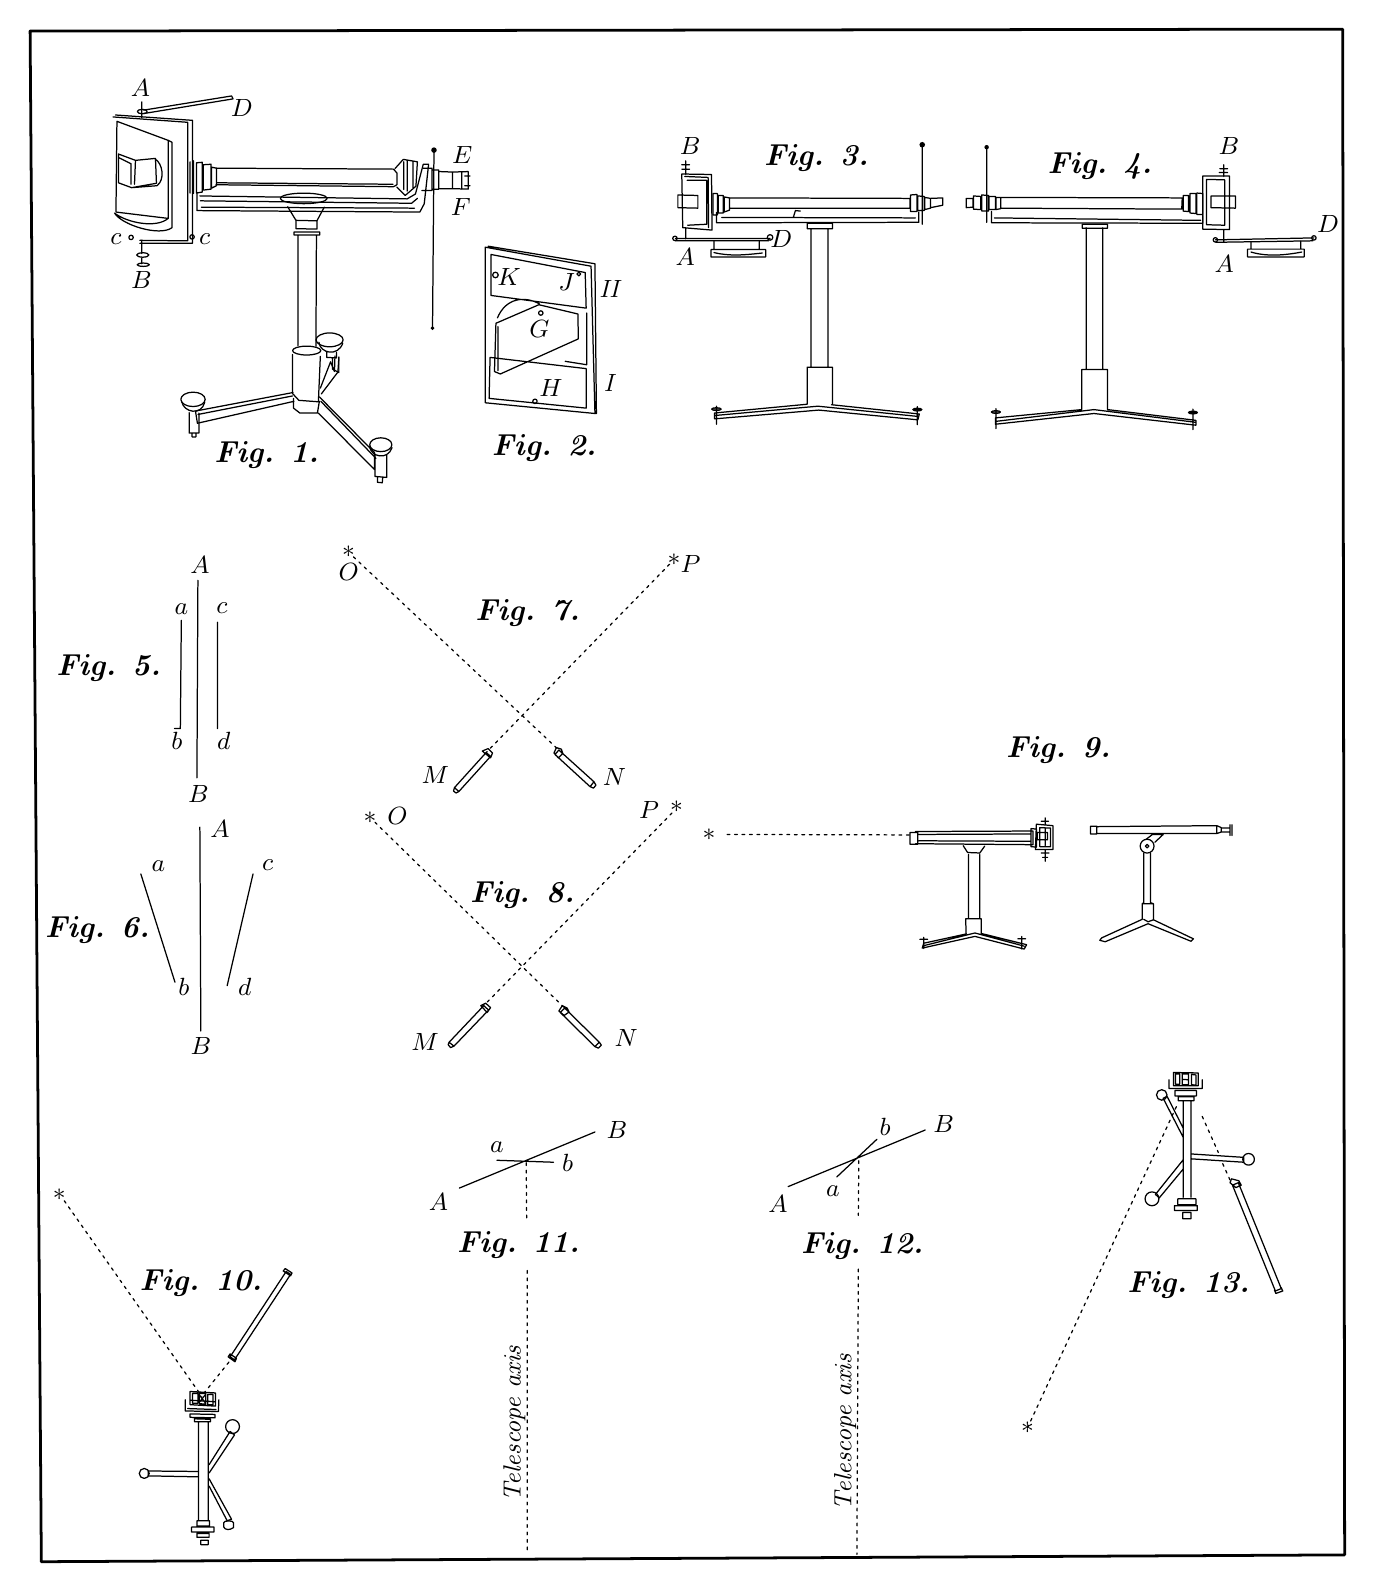
\begin{tikzpicture}[x=.0062cm,y=-.0062cm,line cap=round,line join=round,line width=.45pt,
  every node/.style={font=\fontsize{9}{10}\selectfont\itshape,inner sep=0pt},
  ray/.style={line width=.45pt,dash pattern=on 1pt off 1.7pt},
  caption/.style={font=\fontsize{11}{12}\selectfont\bfseries\itshape}]
\path[use as bounding box] (30,415) rectangle (2735,3560);
\draw[line width=1pt] (35,422)--(2726,418)--(2730,3546)--(58,3560)--cycle;
% Figures 1 and 2: perspective instrument and its mirror system.
\begin{scope}[shift={(110,500)}]
\draw (95,98)--(248,109)--(248,352)--(150,351)
 (100,94)--(258,105)--(258,357)--(150,357)
 (103,107)--(208,146)--(208,306)--(101,293)--cycle;
\draw (98,295)..controls (112,319) and (190,344)..(216,325)--(216,150)--(208,146)
 (98,295)..controls (123,315) and (184,327)..(208,306);
\draw (106,174)--(141,187)--(182,183)--(184,234)--(133,243)--(106,233)--cycle
 (141,187)--(139,236) (106,181)--(132,194)--(132,236)
 (181,184)..controls (197,193) and (202,227)..(185,239)--(133,243);
\draw (154,67)--(154,100) (158,84)--(338,55)--(341,61)--(158,91)
 (154,351)--(154,378) (154,387)--(154,399);
\draw (155,87) ellipse[x radius=1.8pt,y radius=.8pt]
 (156,381) ellipse[x radius=2.2pt,y radius=.8pt]
 (157,401) ellipse[x radius=2.2pt,y radius=.6pt];
\draw (132,345) circle[radius=.8pt] (257,344) circle[radius=.8pt];
\node at (151,39) {$A$}; \node at (359,80) {$D$}; \node at (153,432) {$B$};
\node at (101,348) {$c$}; \node at (283,349) {$c$};
\draw (253,190)--(253,254) (260,188)--(260,255)
 (266,192)--(278,191)--(278,252)--(266,254)--cycle
 (280,196)--(296,195)--(296,246)--(280,248)--cycle
 (297,201)--(307,203)--(307,239)--(297,244)--cycle;
\draw (307,203)--(670,205)--(677,213)--(677,237)--(670,241)--(306,237)
 (308,233)--(669,236)
 (673,204)--(690,185)--(719,190)--(716,240)--(694,259)--(677,242)
 (691,190)--(691,247) (698,188)--(698,250) (710,190)--(710,243);
\draw (273,260)--(698,266)--(715,256)--(731,195)--(742,195)--(733,276)--(724,293)--(267,290)--(267,254)
 (274,270)--(707,275)--(719,265) (276,283)--(713,285)
 (731,203)--(749,203)--(749,249)--(728,249)
 (750,207)--(763,207)--(763,246)--(750,246)
 (765,210)--(791,211)--(791,245)--(765,245)
 (791,211)--(823,210)--(823,246)--(791,245)
 (810,211)--(810,246) (816,219)--(827,219) (816,239)--(827,239);
\draw (753,167)--(750,531);
\fill (753,166) circle[radius=1pt] (750,531) circle[radius=.7pt];
\node at (811,177) {$E$}; \node at (808,282) {$F$};
\draw (486,265) ellipse[x radius=8.5pt,y radius=1.9pt];
\draw (453,282)--(470,310)--(513,311)--(528,283)
 (470,310)--(470,327)--(513,328)--(513,311)
 (466,334)--(519,334)--(519,340)--(466,340)--cycle
 (474,341)--(474,567) (512,342)--(511,568)
 (463,585)--(463,665)--(476,679)--(516,682)--(520,589);
\draw (492,577) ellipse[x radius=5.1pt,y radius=1.6pt];
\draw (465,675)--(465,695)--(478,705)--(514,705)--(518,681)
 (464,663)--(264,701)--(268,726)--(466,681)
 (269,708)--(463,670)
 (518,672)--(631,786)--(631,821)--(516,705)
 (521,681)--(634,798)
 (520,654)--(541,600)--(549,620)--(550,588)
 (522,666)--(556,621)--(558,591);
\draw (259,677) ellipse[x radius=4.4pt,y radius=2.6pt]
 (539,555) ellipse[x radius=4.9pt,y radius=2.5pt]
 (644,770) ellipse[x radius=4pt,y radius=2.5pt];
\draw (236,682)..controls (240,704) and (276,711)..(283,683)
 (251,704)--(251,746)--(271,746)--(271,705)
 (257,746)--(257,754)--(265,754)--(265,747)
 (517,560)..controls (520,583) and (556,590)..(566,562)
 (533,580)--(533,591)--(553,592)--(553,581)
 (545,592)--(545,615)--(558,622)--(558,590)
 (621,773)..controls (623,795) and (658,803)..(667,776)
 (632,790)--(632,835)--(656,837)--(656,791)
 (637,836)--(637,847)--(647,848)--(648,836);
\node[caption] at (410,790) {Fig. 1.};
\draw (858,365)--(1075,404)--(1083,706)--(858,684)--cycle
 (864,363)--(1083,399)--(1086,706)--(1083,706)
 (870,380)--(1063,417)--(1065,490)--(870,464)--cycle
 (868,591)--(1065,614)--(1065,695)--(866,675)--cycle
 (880,521)--(968,483)--(1048,502)--(1049,553)--(889,625)--(877,620)--cycle
 (884,528)--(884,618)
 (883,510)..controls (901,468) and (939,465)..(969,481)
 (1066,500)--(1066,606)--(1022,599);
\draw (879,422) circle[radius=1pt] (1050,420) circle[radius=.7pt]
 (972,500) circle[radius=.8pt] (960,681) circle[radius=.8pt];
\node at (907,427) {$K$}; \node at (1025,437) {$J$};
\node at (969,533) {$G$}; \node at (993,653) {$H$};
\node at (1112,450) {II}; \node at (1111,644) {I};
\node[caption] at (979,776) {Fig. 2.};
\end{scope}
% Figures 3 and 4: the two separately drawn positions with hanging level.
\begin{scope}[shift={(1310,600)}]
\draw (61,115)--(122,116)--(123,230)--(63,225)--cycle
 (67,120)--(115,122)--(116,225) (72,128)--(112,128)--(112,218)--(73,220)
 (53,158)--(94,159)--(94,185)--(53,184)--cycle
 (69,88)--(69,116) (61,96)--(77,96) (61,105)--(77,105)
 (69,225)--(69,248) (48,247)--(242,247) (48,252)--(239,252);
\draw (47,247) circle[radius=.8pt] (242,245) circle[radius=1pt];
\draw (127,252)--(127,270) (220,253)--(220,269)
 (121,270)--(233,270)--(233,285)--(121,285)--cycle
 (127,276)..controls (159,284) and (190,281)..(226,277);
\node at (68,285) {$A$}; \node at (78,57) {$B$}; \node at (265,248) {$D$};
\draw (125,155)--(134,155)--(134,199)--(125,199)--cycle
 (136,159)--(146,159)--(146,195)--(136,195)--cycle
 (148,162)--(159,164)--(159,189)--(148,193)--cycle
 (159,164)--(529,165)--(529,185)--(159,185)
 (132,194)--(132,215)--(547,214)--(547,193)
 (143,204)--(540,205) (290,203)--(294,190)--(304,191)
 (530,158)--(543,157)--(543,192)--(530,192)--cycle
 (545,160)--(558,161)--(558,190)--(545,190)--cycle
 (559,163)--(571,165)--(571,185)--(559,188)--cycle
 (571,165)--(596,164)--(596,179)--(571,184)
 (554,55)--(554,218);
\fill (554,55) circle[radius=1pt];
\draw (318,216)--(370,216)--(370,227)--(318,227)--cycle
 (326,227)--(326,510) (361,227)--(361,510)
 (318,511)--(370,511)--(370,588)
 (318,511)--(318,587)--(128,605)--(128,617)--(342,599)--(545,619)--(548,607)--(368,588)
 (130,610)--(340,591)--(545,612)
 (132,591)--(132,628) (123,597)--(141,597)
 (544,592)--(544,629) (535,598)--(553,598);
\draw (132,597) ellipse[x radius=1.7pt,y radius=.5pt]
 (544,598) ellipse[x radius=1.6pt,y radius=.5pt];
\node[caption] at (337,83) {Fig. 3.};
\draw (644,165)--(658,165)--(658,183)--(644,184)--cycle
 (659,160)--(674,161)--(674,188)--(659,187)--cycle
 (676,158)--(690,159)--(690,191)--(676,191)--cycle
 (691,161)--(704,161)--(704,188)--(691,188)--cycle
 (705,163)--(715,163)--(715,186)--(705,188)--cycle
 (715,163)--(1087,164)--(1086,187)--(715,185)
 (1089,159)--(1100,159)--(1100,192)--(1089,191)--cycle
 (1103,155)--(1115,155)--(1115,196)--(1103,195)--cycle
 (1117,154)--(1129,155)--(1129,198)--(1117,198)--cycle
 (702,205)--(1125,210) (696,192)--(696,215)--(1129,216)--(1129,200)
 (686,60)--(686,214);
\fill (686,60) circle[radius=.8pt];
\draw (1129,119)--(1184,119)--(1184,229)--(1129,228)--cycle
 (1137,126)--(1174,127)--(1174,220)--(1137,219)--cycle
 (1146,160)--(1196,160)--(1196,185)--(1146,184)--cycle
 (1172,96)--(1172,120) (1164,104)--(1180,104) (1163,112)--(1180,112)
 (1172,230)--(1172,253) (1155,250)--(1357,246) (1156,255)--(1355,252);
\draw (1155,250) circle[radius=.8pt] (1357,246) circle[radius=.8pt];
\draw (1228,254)--(1228,269) (1330,253)--(1330,269)
 (1221,269)--(1337,269)--(1337,285)--(1221,285)--cycle
 (1228,275)..controls (1265,286) and (1305,280)..(1332,275);
\node at (1173,300) {$A$}; \node at (1183,57) {$B$}; \node at (1386,217) {$D$};
\draw (882,218)--(934,218)--(934,226)--(882,226)--cycle
 (890,225)--(890,515) (924,225)--(924,515)
 (881,516)--(934,516)--(934,598)
 (881,516)--(881,598)--(704,615)--(704,628)--(906,606)--(1115,630)--(1115,620)--(934,598)
 (706,622)--(906,598)--(1114,624)
 (705,596)--(705,637) (696,603)--(714,603)
 (1109,597)--(1109,639) (1100,604)--(1118,604);
\draw (705,603) ellipse[x radius=1.6pt,y radius=.5pt]
 (1109,604) ellipse[x radius=1.6pt,y radius=.5pt];
\node[caption] at (918,98) {Fig. 4.};
\end{scope}
% Figures 5 and 6: finite, unequal line segments without arrows.
\begin{scope}[shift={(70,1470)}]
\draw (309,78)--(307,483) (275,160)--(273,382)--(261,382) (349,164)--(349,382);
\node at (313,47) {$A$}; \node at (310,516) {$B$};
\node at (275,137) {$a$}; \node at (266,408) {$b$};
\node at (358,135) {$c$}; \node at (362,408) {$d$};
\node[caption] at (126,257) {Fig. 5.};
\draw (313,584)--(315,1002) (192,680)--(262,902) (422,680)--(369,909);
\node at (354,587) {$A$}; \node at (315,1033) {$B$};
\node at (228,663) {$a$}; \node at (280,912) {$b$};
\node at (452,661) {$c$}; \node at (405,912) {$d$};
\node[caption] at (103,795) {Fig. 6.};
\end{scope}
% Figures 7 and 8: crossing rays and two separate telescopes in each figure.
\begin{scope}[shift={(650,1450)}]
\node at (38,40) {$\ast$}; \node at (705,55) {$\ast$};
\node at (38,80) {$O$}; \node at (739,64) {$P$};
\draw[ray] (48,50)--(469,446) (696,65)--(320,451);
\draw (255,523)--(320,451)--(329,459)--(264,531)--cycle
 (312,448)--(324,443)--(333,452)--(329,462)--cycle
 (255,523)--(253,530)--(258,534)--(264,531)
 (469,446)--(541,511)--(533,521)--(461,455)--cycle
 (464,441)--(474,444)--(477,453)--(468,462)--(459,452)--cycle
 (541,511)--(545,518)--(540,524)--(533,521);
\node at (216,497) {$M$}; \node at (583,501) {$N$};
\node[caption] at (405,165) {Fig. 7.};
\node at (82,584) {$\ast$}; \node at (710,563) {$\ast$};
\node at (138,582) {$O$}; \node at (654,568) {$P$};
\draw[ray] (92,594)--(481,975) (701,575)--(315,970);
\draw (244,1045)--(315,970)--(325,979)--(254,1053)--cycle
 (309,970)--(319,965)--(329,974)--(322,984)--cycle
 (244,1045)--(242,1050)--(247,1056)--(254,1053)
 (481,975)--(552,1045)--(543,1054)--(472,984)--cycle
 (476,970)--(486,975)--(490,983)--(480,990)--(469,981)--cycle
 (552,1045)--(556,1051)--(550,1057)--(543,1054);
\node at (195,1044) {$M$}; \node at (607,1036) {$N$};
\node[caption] at (394,743) {Fig. 8.};
\end{scope}
% Figure 9: heliotrop and auxiliary telescope, separately elevated.
\begin{scope}[shift={(1380,1820)}]
\node at (47,250) {$\ast$}; \draw[ray] (84,249)--(459,250);
\draw (459,245)--(475,245)--(475,269)--(459,269)--cycle
 (470,243)--(711,242)--(711,270)--(470,268)
 (477,249)--(705,248) (477,262)--(705,263)
 (707,237)--(718,238)--(718,275)--(707,274)--cycle
 (718,228)--(752,231)--(752,280)--(716,280)--cycle
 (725,235)--(747,236)--(747,274)--(725,274)--cycle
 (736,237)--(736,272) (720,245)--(741,245)--(741,260)--(720,260)--cycle
 (736,215)--(736,229) (728,222)--(743,222)
 (736,280)--(736,304) (728,287)--(744,287) (731,296)--(741,296);
\draw (568,272)--(577,286)--(602,287)--(612,273)
 (579,290)--(579,422) (602,290)--(602,422)
 (573,422)--(605,422)--(605,452)--(698,475)--(693,484)--(592,458)--(484,482)--(487,472)--(574,453)--cycle
 (487,477)--(592,451)--(693,478)
 (487,460)--(487,483) (479,464)--(495,464)
 (688,458)--(688,484) (680,463)--(696,463);
\draw (829,232)--(842,232)--(842,248)--(829,248)--cycle
 (841,233)--(1088,231)--(1088,247)--(841,247)
 (1088,231)--(1097,235)--(1097,244)--(1088,247)
 (1097,236)--(1115,236)--(1115,244)--(1097,244)
 (1115,229)--(1115,251) (1119,229)--(1119,251)
 (961,265)--(978,249)--(956,249)--(943,259);
\draw (945,273) circle[radius=2.5pt] (945,273) circle[radius=.65pt];
\draw (938,287)--(938,389)--(935,391)--(935,423)--(852,461)--(848,466)--(859,469)--(947,432)--(1035,468)--(1040,463)--(958,424)--(958,391)--(952,389)--(952,287)
 (935,391)--(958,391) (938,423)--(947,428)--(958,424);
\node[caption] at (763,76) {Fig. 9.};
\end{scope}
% Figure 10: end-on instrument, oblique auxiliary telescope and ray.
\begin{scope}[shift={(55,2710)}]
\node at (40,98) {$\ast$};
\draw[ray] (50,110)--(332,511) (336,505)--(393,434);
\draw (390,430)--(505,255)--(514,261)--(399,436)--cycle
 (499,254)--(503,249)--(517,258)--(514,264)--cycle
 (386,430)--(390,424)--(403,433)--(400,440)--cycle;
\draw (308,501)--(360,504)--(360,531)--(308,528)--cycle
 (313,505)--(324,505)--(324,525)--(313,525)--cycle
 (327,505)--(340,505)--(340,527)--(327,526)--cycle
 (344,507)--(355,507)--(355,528)--(344,528)--cycle
 (327,508)--(339,524) (339,508)--(327,523)
 (309,519)--(360,522)
 (298,518)--(298,541)--(366,542)--(367,518)
 (303,536)--(361,538) (308,547)--(359,548)--(359,555)--(308,554)--cycle
 (317,557)--(350,558)--(350,563)--(317,563)--cycle
 (325,563)--(325,765) (345,563)--(345,764);
\draw (325,665)--(222,664)--(222,674)--(325,676)
 (347,651)--(390,583)--(399,590)--(347,668)
 (347,695)--(384,766)--(393,763)--(347,680);
\draw (214,669) circle[radius=1.8pt] (395,573) circle[radius=2.5pt];
\draw (377,770)..controls (377,765) and (397,765)..(397,770)--(397,780)..controls (389,786) and (380,785)..(377,779)--cycle
 (322,766)--(348,766)--(348,777)--(322,777)--cycle
 (311,779)--(357,779)--(357,789)--(311,789)--cycle
 (322,792)--(347,792)--(347,800)--(322,800)--cycle
 (330,806)--(345,806)--(345,815)--(330,815)--cycle;
\node[caption] at (330,278) {Fig. 10.};
\end{scope}
% Figures 11 and 12: the unlike inclinations are retained.
\begin{scope}[shift={(790,2630)}]
\draw (125,164)--(403,49) (202,107)--(318,111);
\node at (82,192) {$A$}; \node at (448,44) {$B$};
\node at (202,80) {$a$}; \node at (347,112) {$b$};
\draw[ray] (262,112)--(263,229) (264,333)--(264,915);
\node[caption] at (246,280) {Fig. 11.};
\node[rotate=90] at (238,647) {Telescope axis};
\draw (799,161)--(1080,45) (899,141)--(981,64);
\node at (778,196) {$A$}; \node at (1118,33) {$B$};
\node at (891,170) {$a$}; \node at (998,38) {$b$};
\draw[ray] (944,108)--(943,220) (943,330)--(940,915);
\node[caption] at (951,282) {Fig. 12.};
\node[rotate=90] at (916,664) {Telescope axis};
\end{scope}
% Figure 13: reverse position, its own oblique ray and auxiliary telescope.
\begin{scope}[shift={(2000,2490)}]
\draw[ray] (385,137)--(80,795) (438,157)--(471,231) (480,254)--(497,292);
\node at (80,796) {$\ast$};
\draw (370,82)--(370,100)--(438,100)--(438,82)
 (379,67)--(430,68)--(430,94)--(379,94)--cycle
 (383,70)--(392,70)--(392,91)--(383,91)--cycle
 (397,70)--(410,70)--(410,92)--(397,92)--cycle
 (397,81)--(410,82)
 (416,71)--(425,72)--(425,93)--(416,92)--cycle
 (382,104)--(426,104)--(426,115)--(382,115)--cycle
 (389,117)--(421,117)--(421,125)--(389,125)--cycle
 (399,125)--(399,323) (415,125)--(415,323)
 (399,200)--(358,120)--(366,116)--(399,181)
 (415,234)--(523,241)--(523,251)--(415,244)
 (399,246)--(342,317)--(350,324)--(399,265);
\draw (355,113) circle[radius=1.9pt] (533,245) circle[radius=2.1pt]
 (335,326) circle[radius=2.5pt];
\draw (388,326)--(425,326)--(425,338)--(388,338)--cycle
 (381,340)--(428,340)--(428,350)--(381,350)--cycle
 (398,354)--(415,354)--(415,367)--(398,367)--cycle
 (500,298)--(588,515)--(600,510)--(512,293)--cycle
 (495,293)--(498,285)--(513,289)--(518,298)--(507,303)--cycle
 (586,513)--(589,520)--(603,515)--(600,508);
\node[caption] at (410,502) {Fig. 13.};
\end{scope}
\end{tikzpicture}
\end{center}
